\section{Model}
%Model - Drawing, equations, linear equations.
The quadcopter system is shown in \autoref{droneDiagram}. 
\begin{figure}[H]
	\centering
	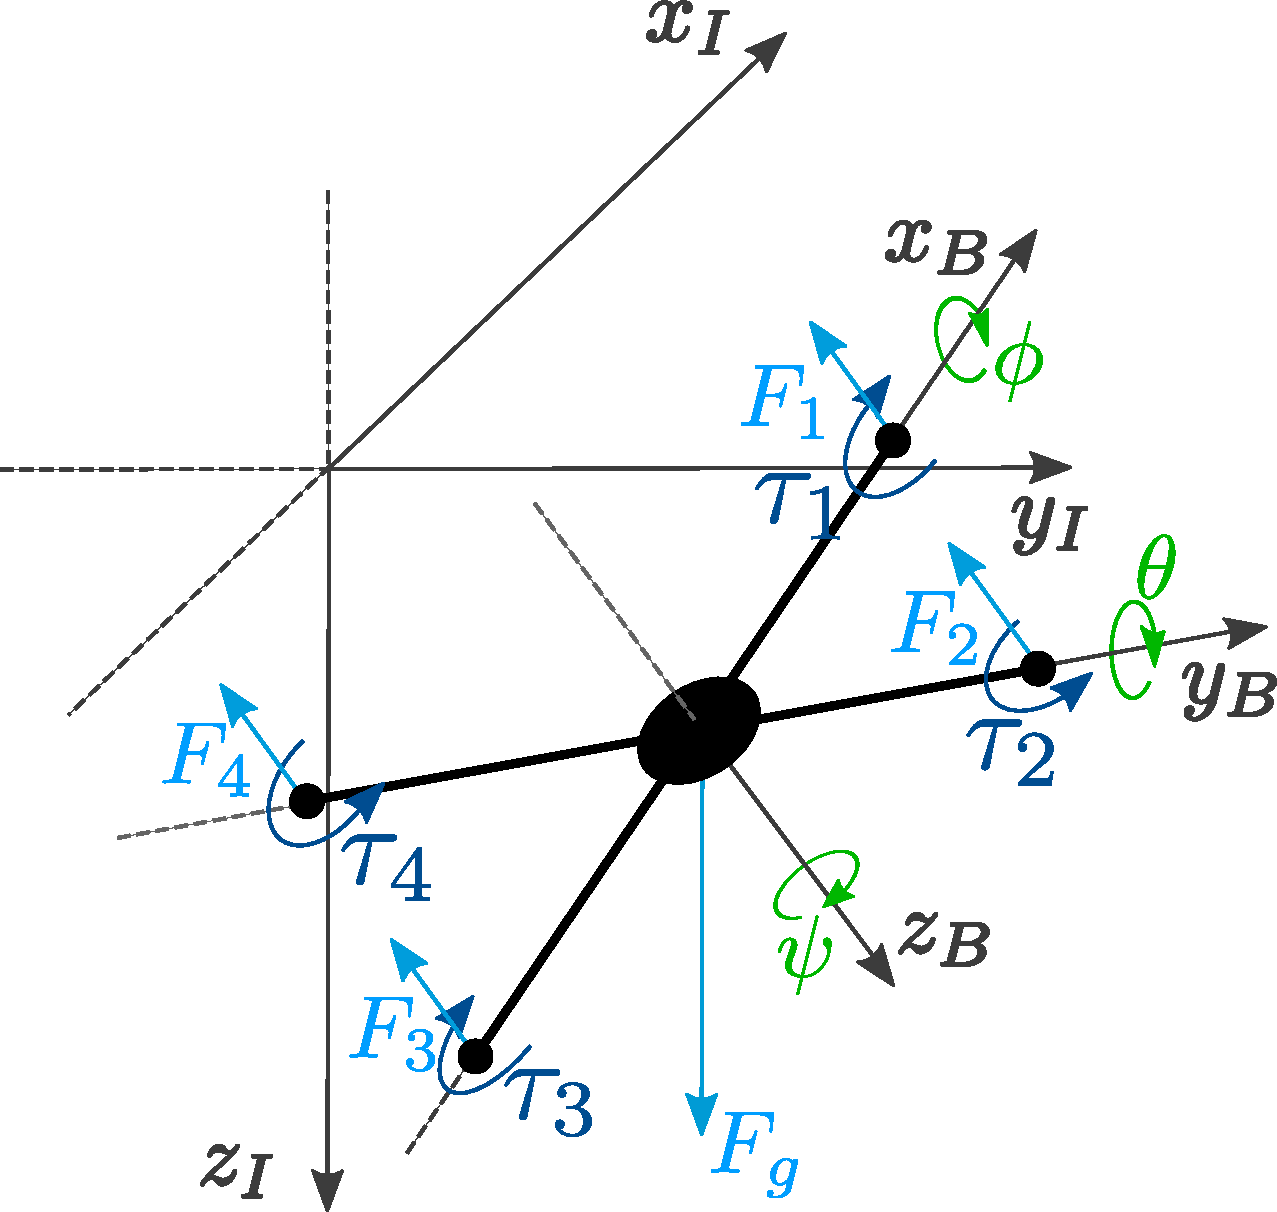
\includegraphics[scale=0.25]{figures/droneDiagram}
	\caption{Quadcopter diagram showing the forces and torques acting on the system and the positive references chosen for rotations and translations in both Inertial and Body coordinate frames.}
	\label{droneDiagram}
\end{figure}
%
As it can bee seen, the system is modeled by using two coordinate frames. The inertial frame is utilized to describe the translational movement while the body frame is attached to the quadcopter and used to characterize its attitude behavior. In the figure, also the positive references for rotational and translational movements are depicted, as well as the main forces and torques acting on the quadcopter. 

The forces generated in the propeller are easily explained in the body coordinate frame. In order to represent them in the inertial frame a rotation matrix is used. It is built considering a 123 rotation sequence \cite{rotationmatrix}.
 
The dynamic model of the quadcopter can be explain through three sets of equations. The first describes the motor and the propeller, the second presents the attitude response of the quadcopter and the third explains how the translational variables of the system evolve.

\subsection{Motor and Propeller}
The four motors in the quadcopter generate a rotation in the propellers that creates the force that lifts the quadcopter. This force is called thrust force and can be modeled as proportional to the square of the motor rotational velocity. The coefficient for this equation is called thrust coefficient and has been found through experiments.  
This rotation also generates a torque on each motor due to drag between air and propeller. Drag torque is compensated in the quadcopter by having two of the motors turning in one direction and the two others in the opposite. It can also be described as proportional to the square of the velocity by terms of a drag coefficient that has also been obtained through tests.
\autoref{eq:thrustForce} and \ref{eq:dragTorque} show the expression for the thrust force and drag torque caused by the rotation of the propeller.
%
\begin{flalign}
	F&=k_{th}\omega^2\label{eq:thrustForce}\\
	\tau&=k_{d}\omega^2\label{eq:dragTorque}
\end{flalign}

Where $F$ is the thrust force, $k_{th}$ is the thrust coefficient, $\omega$ is the angular speed of the motor, $\tau$ is the drag torque and $k_d$ is the drag coefficient.
%\begin{where}
%  \va{F}{is the thrust force}{N}
%  \va{k_{th}}{is the thrust coefficient}{N\  s^2 \  rad^{-2}}
%  \va{\omega}{is the angular velocity}{rad s^-1}
%  \va{\tau}{is the drag torque}{N m}
%  \va{k_d}{is the drag coefficient}{N \  m\  s^2 \  rad^{-2}}
%\end{where}

This equations are used in the attitude and translational models derived below.
%
\subsection{Attitude Model}
The attitude model equations are based on Newton's Second Law for rotational movement and are represented in  \autoref{eq:AngleEqVelocities1}, \ref{eq:AngleEqVelocities2} and \ref{eq:AngleEqVelocities3}. 
%
\begin{flalign}
	J_x\ddot{\phi}&=k_{th} (\omega^2_4-\omega^2_2)  L \label{eq:AngleEqVelocities1}\\
	J_y \ddot{\theta}&=k_{th} (\omega^2_1-\omega^2_3)  L \label{eq:AngleEqVelocities2} \\
	J_z\ddot{\psi}&=k_d (\omega^2_1-\omega^2_2+\omega^2_3-\omega^2_4)\label{eq:AngleEqVelocities3}
\end{flalign}

Where $J_x$, $J_y$ and $J_z$ are the moments of inertia around the three axis of rotation, $\ddot{\phi}$, $\ddot{\theta}$ and $\ddot{\psi}$ are the accelerations in roll, pitch and yaw angles respectively, $\omega_i$ is the rotational speed of each motor and $L$ is the distance between the center of the quadcopter and the position of the motors.

The expressions above state how the thrust force difference between motors 1 and 3 affects the roll angular acceleration, how that between motors 4 and 2 affects the pitch angle and how the yaw acceleration depends on the four motors by means of the drag torques generated on the propellers.  
\subsection{Translational Model}
The equations describing the response of the system along the x, y and z axes is derived from Newton's Second Law. The forces that act on the system are those from the propellers and the gravitational one. These expressions are shown in \autoref{eq:AccelerationEqInertial1}, \ref{eq:AccelerationEqInertial2} and \ref{eq:AccelerationEqInertial3}.
%
\begin{flalign}
     m\ \ddot{x}_I = &-k_{th}\ ({\omega_1}^2+{\omega_2}^2+{\omega_3}^2+{\omega_4}^2) \nonumber\\
     & \cdot (\cos(\phi)\ \sin(\theta)\ \cos(\psi) + \sin(\phi)\ sin(\psi))   \label{eq:AccelerationEqInertial1}\\
     m\ \ddot{y}_I = &-k_{th}\ ({\omega_1}^2+{\omega_2}^2+{\omega_3}^2+{\omega_4}^2)\nonumber\\
     & \cdot (\cos(\phi)\ \sin(\theta)\ \sin(\psi) - \sin(\phi)\ \cos(\psi))  \label{eq:AccelerationEqInertial2}\\
     m\ \ddot{z}_I = &F_g-k_{th}\ ({\omega_1}^2+{\omega_2}^2+{\omega_3}^2+{\omega_4}^2)\nonumber\\
     & \cdot \cos(\phi)\ \cos(\theta)
     \label{eq:AccelerationEqInertial3}
\end{flalign}

Where $m$ is the mass of the quadcopter, $\ddot{x}$, $\ddot{y}$ and $\ddot{z}$ are the accelerations in the directions of the inertial reference frame, $\phi$, $\theta$ and $\psi$ are the roll, pitch and yaw angles respectively and $F_g$ if the gravitational force.

It is worth mentioning that, as the thrust forces always point in the negative z direction in the body coordinate frame, the accelerations in x and y directions in the inertial frame are zero as long as pitch and roll angles are 0.
\subsection{Linearization}
The linearization of the model equations has been developed following the first order Taylor approximation around an equilibrium point of the system. The chosen point is the hovering position and that implies that all variables have a value of zero, that is, the translational and attitude accelerations, velocities and positions. Choosing a zero acceleration equilibrium point along the Inertial z axis yields a equilibrium rotational speeds so that the necessary thrust is generated to compensate for the gravitational force.
\begin{flalign}
    \overline{\omega}_i=\sqrt{\frac{m\  g}{4k_{th}}}
    \label{eq:equilibriumomegas}
\end{flalign}
The resulting equations for the attitude model after the linearization are shown in \autoref{eqAngleLin1}, \ref{eqAngleLin2} and \ref{eqAngleLin3}. 
\begin{flalign}
  J_x\ \Delta\ddot{\phi}   = \ &2\ k_{th}\ L\ {\overline{\omega}_4}\ \Delta \omega_4\ -\ 2\ k_{th}\ L\ {\overline{\omega}_2}\ \Delta \omega_2
  \label{eqAngleLin1} \\
  J_y\ \Delta\ddot{\theta} = \ &2\ k_{th}\ L\ \overline{\omega}_1\ \Delta \omega_1\ -\ 2\ k_{th}\ L\ \overline{\omega}_3\ \Delta \omega_3
  \label{eqAngleLin2} \\
  J_z\ \Delta\ddot{\psi}   = \ &2\ k_d\ {\overline{\omega}_1}\ \Delta \omega_1\ -\ 2\ k_d\ {\overline{\omega}_2}\ \Delta \omega_2\ \nonumber 
  \\ & +\ 2\ k_d\ {\overline{\omega}_3}\ \Delta \omega_3\ -\ 2\ k_d\ {\overline{\omega}_4}\ \Delta \omega_4 \label{eqAngleLin3}
\end{flalign}

Where $\Delta\ddot{\phi}$, $\Delta\ddot{\theta}$ and $\Delta\ddot{\psi}$ are the changes in rotational acceleration from equilibrium, $\overline{\omega}_i$ is the rotational speed of each motor in equilibrium and $\Delta \omega_i$ is the change in rotational speed of each motor from equilibrium. 

Similarly, the equations of the translational model are linearized. The result is shown in \autoref{eq:TransLinearEquations1}, \ref{eq:TransLinearEquations2} and \ref{eq:TransLinearEquations3}.
\begin{flalign}
  m\ \Delta\ddot{x}_I =\ &-k_{th}\ ({\overline{\omega}_1}^2+{\overline{\omega}_2}^2+{\overline{\omega}_3}^2+{\overline{\omega}_4}^2)\  \Delta\theta \label{eq:TransLinearEquations1} \\
  m\ \Delta\ddot{y}_I =\ & k_{th}\ ({\overline{\omega}_1}^2+{\overline{\omega}_2}^2+{\overline{\omega}_3}^2+{\overline{\omega}_4}^2)\ \Delta\phi \label{eq:TransLinearEquations2}\\
  m\ \Delta\ddot{z}_I =\ &-2\ k_{th}\ \overline{\omega}_1\ \Delta\omega_1 -2\ k_{th}\ \overline{\omega}_2\ \Delta\omega_2 \nonumber \\
  &-2\ k_{th}\ \overline{\omega}_3\ \Delta\omega_3-2\ k_{th}\ \overline{\omega}_4\ \Delta\omega_4\ \label{eq:TransLinearEquations3}
\end{flalign} 
Where $\Delta\ddot{x_I}$, $\Delta\ddot{y_I}$ and $\Delta\ddot{z_I}$ are the changes in linear acceleration from equilibrium in each direction of the inertial frame and $\Delta \phi$ and $\Delta \theta$ are the changes in roll and pitch from equilibrium respectively.